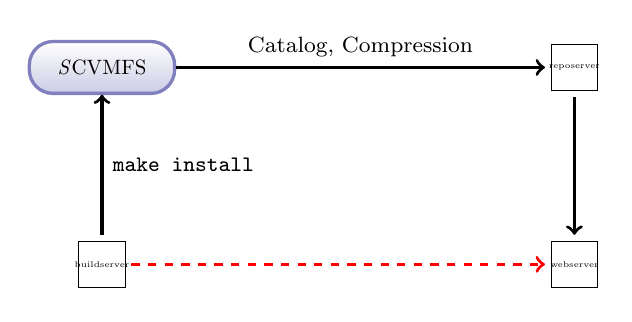
\begin{tikzpicture}
      [block/.style={
         rectangle,
         very thick,
         rounded corners=3mm,
         minimum width=\blockwidth,
         minimum height=\blockheight},
      fuse/.style={
         block,
         draw=blue!50!black!50,
         top color=white,
         bottom color=blue!50!black!20},
      legend/.style={
      	font=\footnotesize},
      every node/.style={
      	anchor=center}]
         \edef\blockwidth{7em} 
	\edef\blockheight{2.5em}
                  
	\node[scale=0.6] (buildserver) at (0,0) {\pgfimage{buildserver}};
	\node[scale=0.75,fuse] (scvmfs) at (0,2.5) {\emph{S}CVMFS};
	\node[scale=0.6] (reposerver) at (6,2.5) {\pgfimage{reposerver}};
	\node[scale=0.6] (webserver) at (6,0) {\pgfimage{webserver}};
	
	\draw[->, very thick] (buildserver.north) -- node[legend,right]{\texttt{make install}} (scvmfs.south);
	\draw[->, very thick] (scvmfs.east) -- node[legend,above]{Catalog, Compression} (reposerver.west);
	\draw[->, very thick] (reposerver.south) -- (webserver.north);
	\draw[->, very thick, dashed, red] (buildserver.east) -- (webserver.west);
	
	%\draw[->, very thick] (buildserver.east)
	% -- node[legend,right]{\texttt{make install}}
	%                                    node[scale=0.75,fuse, above] {\emph{S}CVMFS} (0,2.5);
	%\draw[->, very thick] (2.5,2.5) -- node[legend,above]{Catalog, Compression} (6,2.5) 
	%                                    node[right] {\includegraphics[scale=0.6]{reposerver}};
\end{tikzpicture}